\section{Idiotpage}
\subsection{Derivation Rules}

{\setlength{\extrarowheight}{4pt}
	\begin{tabular}{@{}lcl@{}}
		\textbf{f(x)} & $\rightarrow$ & \textbf{f'(x)} \\
		\toprule
		$c$ & $\rightarrow$ & $0$ \\
		$x^n$  & $\rightarrow$ & $n\cdot x^{n-1}$ \\
		$c\cdot g\left(x\right)$  & $\rightarrow$ & $c\cdot g'\left(x\right)$ \\
		$e^x$  & $\rightarrow$ & $e^x$ \\
		$a^x$ & $\rightarrow$ & $a^x\ln(a)$\\
		\midrule
		$g\left(x\right)+h\left(x\right)$  & $\rightarrow$ & $g'\left(x\right)+h'\left(x\right)$ \\
		$u\left(x\right)\cdot v\left(x\right)$  & $\rightarrow$ & $u'\left(x\right)\cdot v\left(x\right)+u\left(x\right)\cdot v'\left(x\right)$ \\ 
		$\frac{u\left(x\right)}{v\left(x\right)}$  & $\rightarrow$ & $\frac{u'\left(x\right)\cdot v\left(x\right)-u\left(x\right)\cdot v'\left(x\right)}{v^2\left(x\right)}$ \\
		$u\left(v\left(x\right)\right)$  & $\rightarrow$ & $u'\left(v\left(x\right)\right)\cdot v'\left(x\right)$ \\
		\midrule
		$\cos\left(x\right)$ & $\rightarrow$ & $-\sin(x)$ \\
		$\sin\left(x\right)$ & $\rightarrow$ & $\cos(x)$ \\	
		$\cosh\left(x\right)$ & $\rightarrow$ & $\sinh(x)$ \\
		$\sinh\left(x\right)$ & $\rightarrow$ & $\cosh(x)$ \\
		$\tan\left(x\right)$ & $\rightarrow$ & $\frac{1}{\cos^2(x)} = 1 + \tan^2(x)$ \\	
		$\ln\left(x\right)$ & $\rightarrow$ & $\frac{1}{x}$ \\
		$f^{-1}\left(x\right) {\scriptscriptstyle (Umkehrf.)}$  & $\rightarrow$ & $\frac{1}{f'(f^{-1}(x))}$ \\
		$\left|x\right|$ & $\rightarrow$ & $\frac{\left|x\right|}{x}$ \\
		\midrule
		$\sigma(x) = \frac{1}{1+ e^{-xc}}$ & $\rightarrow$ & $\sigma(x)(1 - \sigma(x)$\\
	\end{tabular}
}

\subsubsection{Unit circle}
\begin{center}
	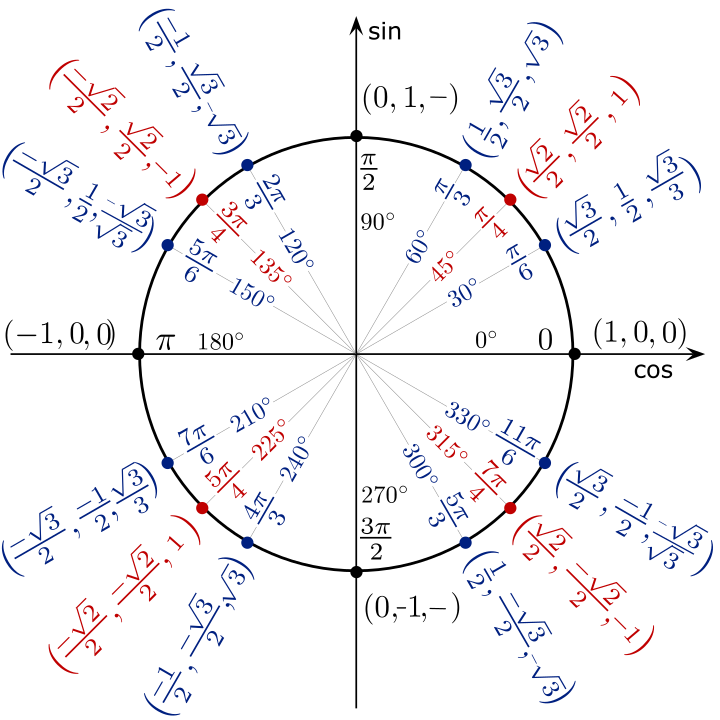
\includegraphics[width=0.8\columnwidth]{Images/einheitskreis}\\
	Punkte auf Kreis [$\cos(\alpha), \sin(\alpha), \tan(\alpha)$]
\end{center}

\subsubsection{Periodicity}
$\cos(a+k\cdot2\pi)=\cos(a) \qquad \sin(a+k\cdot2\pi)=\sin(a) \qquad
(k \in \mathbb{Z})$

\subsubsection{Double and Half angle}	
\begin{align*}
	\sin(2a) &=2\sin(a)\cos(a) &= \frac{2\tan(a)}{1 +\tan^2(a)}\\
	\cos(2a) &=\cos^2(a)-\sin^2(a) &= 2\cos^2(a)-1 &= 1-2\sin^2(a)\\
	\cos^2 \left(\frac{a}{2}\right) &=\frac{1+\cos(a)}{2} \\
	\sin^2 \left(\dfrac{a}{2}\right)&=\frac{1-\cos(a)}{2}
\end{align*}


\subsubsection{Addition Theorems}
\begin{align*}
	\sin(a \pm b)&=\sin(a) \cdot \cos(b) \pm \cos(a) \cdot \sin(b)\\
	\cos(a \pm b)&=\cos(a) \cdot \cos(b) \mp \sin(a) \cdot \sin(b)\\	
	\tan(a \pm b)&=\dfrac{\tan(a) \pm \tan(b)}{1 \mp \tan(a) \cdot \tan(b)}\\
	\sin(a)+\sin(b) &= 2\sin\left(\frac{a + b}{2}\right)\cos\left(\frac{a - b}{2}\right)\\
	\sin(a)-\sin(b) &= 2\cos\left(\frac{a + b}{2}\right)\sin\left(\frac{a - b}{2}\right)\\
	\cos(a)+\cos(b) &= 2\cos\left(\frac{a + b}{2}\right)\cos\left(\frac{a - b}{2}\right)\\
	\cos(a)-\cos(b) &= -2\sin\left(\frac{a + b}{2}\right)\sin\left(\frac{a - b}{2}\right)\\
	\sin(a)\sin(b)&=\frac{1}{2}(\cos(a-b)-\cos(a+b))\\
	\cos(a)\cos(b)&=\frac{1}{2}(\cos(a-b)+\cos(a+b))\\
	\sin(a)\cos(b)&=\frac{1}{2}(\sin(a-b)+\sin(a+b))\\
\end{align*}

\subsubsection{Potencies}
\begin{align*}
	\sin^2(a) &= \frac{1}{2}(1 - \cos(2a)) \\
	\sin^3(a) &= \frac{1}{4}(3\sin(a) - \sin(3a)) \\
	\cos^2(a) &= \frac{1}{2}(1 + \cos(2a)) \\
	\cos^3(a) &= \frac{1}{4}(3\cos(a) + \cos(3a)) \\
\end{align*}

